\section{Allgemeines über Pointer}

Pointer nennt man auch \begriff{Zeiger}, \begriff{Verweise} oder \begriff{Datenreferenzen}. Ein Pointer ist ein Verweis bzw. eine Referenz auf ein Zielobjekt/Zeigerziel/Target eines festgelegten Datentyps. In den folgenden Darstellungen ist:
\begin{center}
	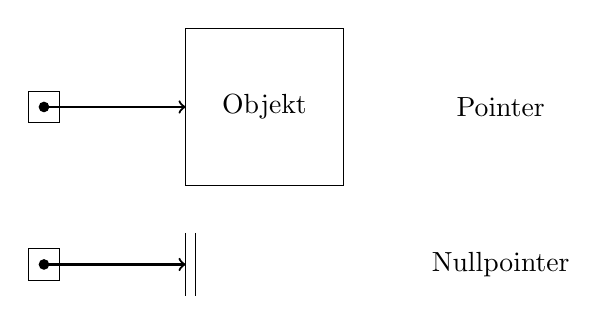
\begin{tikzpicture}[scale=0.2]
		\draw (0,0) -- (2,0);
		\draw (0,0) -- (0,2);
		\draw (2,0) -- (2,2);
		\draw (0,2) -- (2,2);
		\draw[fill = black] (1,1) circle (0.3);
		\draw[->, thick] (1,1) -- (10,1);
		\draw (10,-4) -- (10,6);
		\draw (10,-4) -- (20,-4);
		\draw (10,6) -- (20,6);
		\draw (20,-4) -- (20,6);
		\node at (15,1) (n) {Objekt};
		\node at (30,1) (n2) {Pointer};
		
		\draw (0,-10) -- (2,-10);
		\draw (0,-10) -- (0,-8);
		\draw (2,-10) -- (2,-8);
		\draw (0,-8) -- (2,-8);
		\draw[fill = black] (1,-9) circle (0.3);
		\draw[->, thick] (1,-9) -- (10,-9);
		\draw (10,-7) -- (10,-11);
		\draw (10.6,-7) -- (10.6,-11);
		\node at (30,-9) (n2) {Nullpointer};
	\end{tikzpicture}
\end{center}

Ein Pointer hat zu Beginn der Programmausführung einen undefinierten Zustand, der nicht als solcher erkannt werden kann. Die Verwendung eines solchen Pointers kann große Probleme verursachen.

Zeiger sind kein eigenständiger Typ, sondern nur mit dem Attribut \texttt{pointer} gekennzeichnet:
\begin{lstlisting}
! eine normale Variable
integer :: variable
! ein Pointer
integer, pointer :: ptr
\end{lstlisting}

Zeiger sind streng typisiert, das heißt man kann nur auf Objekte zeigen, deren Typ identisch mit dem Zeigertyp ist. Es gibt also keine Universalpointer. Der Pointer im oberen Quelltext kann also nur auf Variablen mit dem Typ \texttt{integer} zeigen.

Jedes beliebige Objekt vom passenden Objekttyp kann als Ziel eines Zeigers dieses Typs verwendet werden, wenn die Zielvariable das Attribut \texttt{target} trägt oder das Objekt ein dynamisches im Heap erzeugtes Objekt ist.
\begin{lstlisting}
integer, target :: ziel
integer, pointer :: ptr
\end{lstlisting}

Jede Pointer-Variable kann als Zeigerziel dienen. Ohne \texttt{target}-Attribut.

Implizit werden Pointer immer automatisch dereferenziert, außer in den Anweisungen \texttt{nullify()}, \texttt{allocate()}, \texttt{deallocate()}, der Pointer-Zuweisung \texttt{pointer => ziel} sowie in der \texttt{associated}-Abfragefunktion.

Pointer sind in Fortran in der Regel mehr als nur Adressen.

Werfen wir nun nochmal einen Blick auf die Pointer-Kontexte, in denen Pointer automatisch dereferenziert werden.

\begin{*anmerkung}
	Wird gerne in der Klausur abgefragt, steht aber auch in dem zur Klausur zugelassenen Buch des Rechenzentrums Niedersachsen über den Fortran-Standard.
\end{*anmerkung}

\begin{itemize}
	\item Die Funktion \texttt{nullify(p1, p2, ...)} versetzt die Pointer \texttt{p1}, \texttt{p2} und so weiter in den definierten Zustand Null = nicht assoziiert.
	\item \texttt{allocate(p1, p2, ...)} legt Speicherblöcke im Heap für die Zielobjekte der Pointer an und setzt die Pointer als Referenzen auf ihren jeweiligen Speicherblock. Alle Pointer sind im definierten Zustand assoziiert.
	\item Mit \texttt{deallocate(p1, p2, ...)} werden die Speicherblöcke, auf die die Pointer zeigen freigegeben und die Pointer auf Null gesetzt. Der Pointer muss dafür assoziiert und ein ganzen Objekt, also kein Subarray, Substring oder ähnliches, sein.
	\item Pointer werden mit \texttt{ptr => tgt} oder \texttt{ptr1 => ptr2} zugewiesen.
	\item Die Abfragefunktion \texttt{associated()} kann auf recht unterschiedliche Weisen eingesetzt werden:
	\begin{itemize}
		\item \texttt{associated(ptr)} $\to$ \texttt{.true.}, wenn auf ein Ziel gezeigt wird; \texttt{.false.}, wenn \texttt{ptr} auf Null zeigt.
		\item \texttt{associated(ptr, tgt)} $\to$ \texttt{.true.}, wenn \texttt{ptr} auf \texttt{tgt} zeigt, sonst \texttt{.false.}
		\item \texttt{associated(ptr1, ptr2)} $\to$ \texttt{.true.}, wenn beide Pointer denselben Zustand (nicht Null) haben, sonst \texttt{.false.}
	\end{itemize}
\end{itemize}

Wie schon oben angesprochen, ist der Umgang mit Pointern nicht ganz ungefährlich, es gibt einige Gefahren für den Hauptspeicher, insbesondere den Heap.

\begin{*anmerkung}
	auch wichtig in der Klausur, steht aber leider nicht im Buch, muss also auswendig gelernt werden
\end{*anmerkung}

\begin{itemize}
	\item Verwendung eines nicht definierten oder nicht gültigen Pointers in \texttt{deallocate}, \texttt{=>}, \texttt{associated}-Abfragen und normalen (nicht Pointer-) Kontext, das heißt in Expressions, in denen alle Pointer automatisch dereferenziert werden.
	\item \begriff{Dangling Pointer} entstehen, wenn das Zeigerziel verloren geht, z.B. durch \texttt{deallocate} über anderen Pointern oder eines \texttt{allocatable}-Feldes oder wenn das Zielobjekt "'out of scope"' geht, zum Beispiel durch Verlassen seiner Prozedur.
	\item \begriff{Speicherleichen}, Garbage, memory leaks: haben im Prinzip das ewige Leben im Heap, wenn keine Referenzen mehr auf ein Heap-Objekt existiert, über die man es freigeben könnte.
\end{itemize}